\section{Background and Preliminaries}
\label{sec:background}
UPPRESSO is designed to be compatible with OpenID Connect (OIDC) and provide privacy protections based on the discrete logarithm problem. Next, we briefly introduce OIDC and the discrete logarithm problem.

\subsection{OpenID Connect (OIDC)}
\label{subsec:OIDC}
%As an extension of OAuth 2.0 for user authentication,
OIDC is one of the most popular SSO protocols~\cite{OpenIDConnect}. %As other SSO protocols~\cite{SAMLIdentifier}, OIDC
It involves three entities, i.e., {\em users}, the {\em identity provider (IdP)}, and {\em relying parties (RPs)}.
Users and RPs register at the IdP with identifiers %($ID_U$, $ID_{RP}$ and $PID_U$ in some schemes) %(or $PID_{RP}$ in some schemes)
and other necessary information such as credentials and RP endpoints (e.g., the URLs to receive identity proofs).
% below can be removed
The IdP is assumed to maintain these attributes securely.

%\vspace{1mm}
\noindent\textbf{OIDC Implicit Flow.}
OIDC supports three types of user login flows: {\em implicit flow}, {\em authorization code flow} and {\em hybrid flow} (i.e., a mix-up of the previous two).
%In the implicit flow, an {\em id token} is generated as the identity proof, which contains a user identifier, an RP identifier, the issuer (i.e., IdP), the validity period, and other requested attributes. The IdP signs the id token using its private key to ensure integrity, and sends it to the RP through the user.
%In the authorization code flow, the IdP binds an authorization code with the RP, and sends it to the RP through the user; then, the RP establishes an HTTPS connection to the IdP and uses the authorization code with the RP's credential to obtain the user's identifier and other attributes.
UPPRESSO is compatible with all three flows. For brevity, we will present our design and implementation on top of the OIDC implicit flow in the rest of the paper and discuss the extension to support the authorization code flow in Section~\ref{sec:discussion}.

As shown in Figure~\ref{fig:OpenID}, first, the user initiates a login request to an RP. Then, the RP constructs an identity proof request with its identifier, an endpoint to receive the identity proof and a scope of requested user attributes, and sends the request to the user who will redirect it to the IdP. If the user has not been authenticated yet, the IdP initiates an authentication process to authenticate the user based on her identity and credential. If privacy-preserving pseudo-identifier is used, this process also involves mapping $ID_U$ to $PID_U$ based on $ID_{RP}$. Once successfully authenticating the user, the IdP generates an identity proof (called {\em id token}) and returns it to the RP endpoint through user redirection. The id token contains a user identifier ($ID_U$ or $PID_U$), an RP identifier ($ID_{RP}$), the issuer, a validity period, the requested user attributes, etc. If the RP's endpoint has not been registered at the IdP, the IdP will return a warning to notify the user about potential identity proof leakage. Besides redirecting the messages between the RP and the IdP, the user also checks if the RP is permitted to obtain the user attributes in the identify proof. Usually, the redirection and checking actions are handled by a user-controlled software, called {\em user agent} (e.g., browser). Finally, the RP verifies the received identity proof and makes the authentication decision.
%extracts user's identifier and returns the authentication result to the user (Step 7).

%\vspace{1mm}
\noindent\textbf{RP Dynamic Registration.}
OIDC also supports {\em RP dynamic registration}~\cite{DynamicRegistration}. When an RP first registers at an IdP, it obtains a registration token with which the RP can %initiate a dynamic registration process to
update its information (e.g., endpoints) with the IdP in a later time. After a successful dynamic registration, the RP obtains a new $ID_{RP}$ from the IdP.
UPPRESSO leverages this function and slightly modifies the dynamic registration process to implement the {\em $PID_{RP}$ registration} process (see details in Section~\ref{sec:UPPRESSO}.C), which allows an RP to generate different privacy-preserving RP identifiers and register them with the IdP.

\begin{figure}[t]
  \centering
  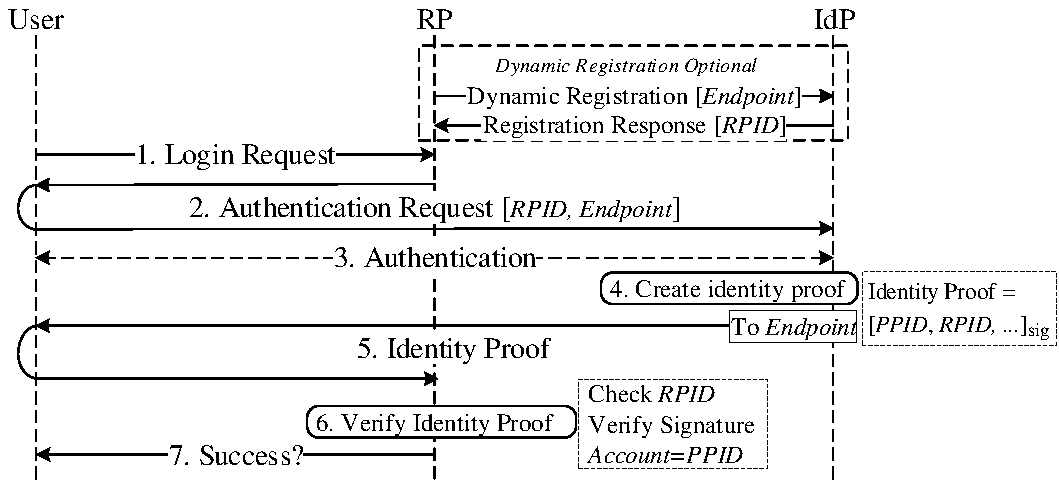
\includegraphics[width=0.95\linewidth]{fig/OIDC1.pdf}
  \caption{The implicit flow of OIDC.}
  \label{fig:OpenID}
\end{figure}


\begin{comment}

\subsection{Discrete Logarithm Problem}
\label{sec:dlp}


Based on the discrete logarithm problem, UPPRESSO designs the identifier-transformation functions. %$\mathcal{F}_{ID_{RP} \mapsto PID_{RP}}$ and $\mathcal{F}_{ID_{U} \mapsto PID_{U}}$ to generate privacy-preserving user identifier (e.g. $PID_U$) and RP identifier (e.g. $PID_{RP}$), respectively.
Here, we briefly review the discrete logarithm problem.
%A number $g$ ($0<g<p$) is called a primitive root modular a prime $p$, if for ${\forall}y$ ($0<y<p$), there is a  number $x$ ($0\le x <p-1$) satisfying $y=g^x \pmod p$.
For the finite field $GF(p)$ where $p$ is a large prime, a number $g$ is called a generator of order $q$, if it constructs a cyclic  group of $q$ elements by calculating $y=g^x \ mod\ p$.
And $x$ is called the discrete logarithm of $y$ modulo $p$. Given a large prime $p$, a generator $g$ and a number $y$, it is computationally infeasible to solve the discrete logarithm (i.e., $x$) of $y$~\cite{WXWM}, which is called the discrete logarithm problem.
The hardness of solving discrete logarithms is utilized to design several secure cryptographic primitives, including Diffie-Hellman key exchange and the digital signature algorithm (DSA).

%In the process of $F_{PID_{RP}}$ and $F_{PID_U}$, we needs to calculate the primitive root for a  large prime $p$ as follows~\cite{Shoup,Wang}. First, we retrieve a primitive root $g_m$  modulo $p$ from all the integers by finding the first integer passing  the primitive root checking.  A lemma is propose to simply the checking, that if $p=2q+1$ ($q$ is a prime),  an integer $\mu \in (1, p-1)$ is a primitive root if and only if $\mu^2\neq 1 \ mod \ p$ and $\mu^q\neq 1 \ mod \ p$. Then, based on $g_m$, we can calculate a new primitive root $g = g_{m}^{t} mod \ p$, where $t$ is an integer coprime to $p-1$.
\end{comment}
